\chapter{Introduction}
\label{chap:introduction}

\minitoc

\graphicspath{{.}{chapitres/introduction/}}

Nowadays software are omnipresent in people's life: banking, e-commerce, communication, etc. 
And the more and more, critical aspects such as aeronautics, voting system or even health care relies on software.

In one of his famous lectures~\cite{DijkstraLecture1989}, Dijkstra has stated that in software: 
\begin{center}
	\emph{``the smallest possible perturbations - \ie changes of a single bit - can have the most drastic consequences.''.}
\end{center}

Dijkstra highlights the fact that a small fault in software might affect lives.
For example, a flight crash happened in 1993 due to an error in the flight-control software of the the Swedish JAS 39 Gripen fighter aircraft.

To avoid such situations, software editors adopted testing philosophies: the tester writes code that verify that the program is doing what the developer expects.
Over the last decade, strong unit testing has become an essential component of any serious software project, whether in industry or academia.
The agile development movement has contributed to this cultural change with the global dissemination of test-driven development techniques~\cite{beck2003test}.
More recently, the DevOps movement has further strengthened the testing practice with an emphasis on continuous and automated testing~\cite{Roche2013Devops}.

However, testing is tedious and costly for industries: there is no direct return to invest.
Thus, developers under pressure or by lack of discipline or time might skip the tests.

To overcome this problem, research investigates the automation of creating strong tests.
Automatic generation of tests has been well studied in the last past years~\cite{ESECFSE11, PachecoE2005}.
The dream was that a command-line would give you a complete test suite, that verifies the whole program.
For free, or almost, all the program would be well-tested.
However, studies show that developers are not using automatic test generation~\cite{TOSEM_userstudy}.
The authors investigate the truthfulness of the following hypothesis:

\emph{generating high coverage test data, we aid testers in constructing test suites capable of detecting faults.}

However, their studies showed that achieving high coverage does not necessarily improve the ability to test software.
The difficulties to understand, integrate and maintain automated test suite prevent the adoption by developers.
Also, most of the tools relies on weak or partial oracles, \eg absence of runtime errors, making them useless against bugs that do not set the program into a wrong state.

In this thesis, I aim at addressing this issue.
More precisely, the ultimate goal of this thesis is to provide an usable tool that assist developers to maintain their test suite, in the context of DevOps and continuous integration.
To do so, I use test suite amplification, which is an emerging field, that derived existing test methods to create variants of them according to an engineering goal.
It means that test suite amplification exploits the knowledge that developers introduced in the seed test method.
This knowledge is a key to obtain usable, valuable and strong test methods.
By construction, test suite amplification's output is close to the test methods used seed, since it is obtained by applying insertions, deletions or modifications on the seed test method.
Which means that for developers that know very-well their software and their test suite, it is easier to understand amplified test method since they share a commons-part with what they developed.

The remaining of this chapter is as follow:

In \autoref{sec:intro:stamp} present the context of the thesis, the H2020 European project \emph{STAMP};

Then, I expose the global vision  of this thesis in \autoref{sec:intro:vision} and its roadmap in \autoref{sec:intro:roadmap};

Eventually, I list the resulting software of this thesis in \autoref{sec:intro:software} and my publications in \autoref{sec:intro:publications}.

\section{STAMP-project}
\label{sec:intro:stamp}

\begin{figure}[h]
	\centering
	\fbox{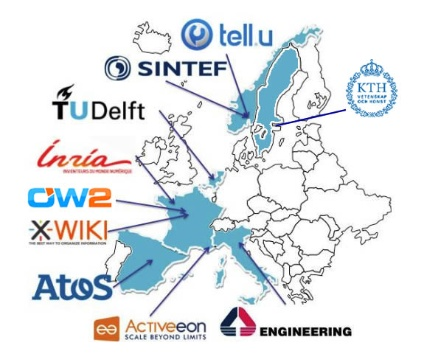
\includegraphics[width=.6\linewidth]{StampConsortiumEUMap.jpg}}
	\caption{STAMP H2020 Project Partners}
	\label{fig:intro:partners-map}
\end{figure}

My thesis takes place within the STAMP project, which is has been funded from the European Union's H2020 research and innovation programme under the grant agreement 731529.

STAMP stands for \textbf{S}oftware \textbf{T}esting \textbf{AMP}lification.
STAMP leverages advanced research in test generation and innovative methods of test amplification to push automation in DevOps one step further.

Test amplification reuses existing test assets and generate more test cases and test configurations at each modification of the application.
The main goal of STAMP techniques are to reduce the number and cost of regression bugs at unit level, configuration level and production stage, by acting at all level of the development cycle.

STAMP will raise confidence and foster adoption of DevOps by the European IT industry.
The project gathers four academic partners with strong software testing expertise, five software companies (in: e-Health, Content Management, Smart Cities and Public Administration), and an open source consortium. 

This industry-near research addresses concrete, business-oriented objectives.

\subsection{Research Directions}
\label{subsec:intro:research-directions}

In STAMP, there are 3 research directions: unit testing amplification, configuration testing amplification and online testing amplification.
These 3 directions are made to be integrated in different step of the Software life-cycle, see \autoref{fig:intro:lifecyle}.

\begin{figure}[h]
	\centering
	\fbox{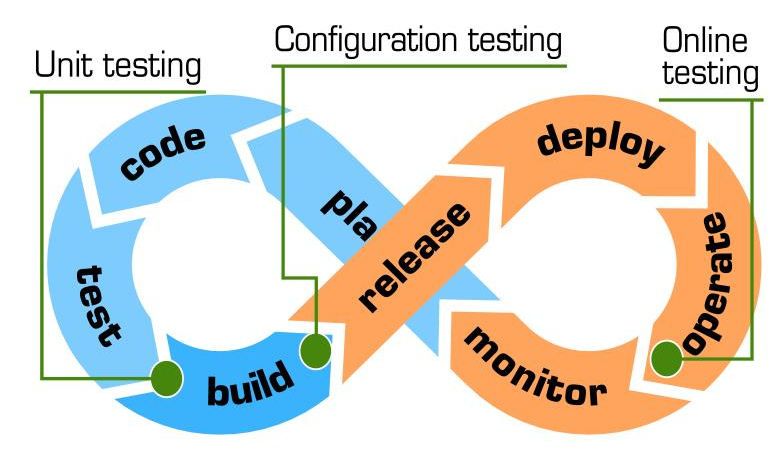
\includegraphics[width=.7\linewidth]{Workshop-intro.jpg}}
	\caption{STAMP's directions integrated in the Software life-cycle.}
	\label{fig:intro:lifecyle}
\end{figure}

\subsubsection{Unit Testing Amplification}
\label{subsubsec:intro:research-directions:unit-test-ampl}

Unit testing refers to testing small and limited part of the Software.
That is to say, it tests a single component, which has, ideally, no interference with others components.
Unit testing is a crucial part of testing since it verifies that every single component of Software does what it is expected to do.

It has two majors benefit:

1) It is easier to test and verify the behavior of a single component;

2) It allows to split the development into small part and view the system as a composition of a lot of small parts.

Unit test amplification aims at generating unit tests that are variants of existing unit tests.
These variants would improve the overall quality of unit tests according to a given engineering goal.

During my thesis, I was mainly involved in this research direction.

\subsubsection{Configuration Testing Amplification}
\label{subsubsec:intro:research-directions:config-ampl}

Configuration testing is the activity of assembling different services in a complete system, to deploy and test it, based on a pre-defined model.
Configuration testing amplification performs automatic amplification of configurations on the model, in the forms of mutation and crossover.
The goal is to create un-tested configuration to stress the Software in newly created environments.

\subsubsection{Online Amplification}
\label{subsubsec:intro:research-directions:online-ampl}

Online test amplification automatically extracts information from logs collected in production in order to generate new tests that can replicate failures, crashes, anomalies and outlier events.
This research directions aims at helping developers to debug the Software in case of crash during the production.
Debugging is a tedious task, and having a unit test method, automatically generated, would save a lot of time.

\subsection{STAMP's Output}

STAMP's final output would be micro-services that allow the developers to use STAMP's tools on their own project.
STAMP envisions a web interface, on which the developers would be able to install, configure and execute the tools.
Also, the developers would be able to manage the output of these executions and link them directly to their project, \eg integrate an amplified unit test into their test suite.

\section{Thesis Vision}
\label{sec:intro:vision}

As this thesis is funded by STAMP, its ultimate goal is correlated to the one of STAMP.
That is to say, this thesis aims at providing a set of tools to assist developers in the test suite evolution.
In particular,  these tools apply test amplification to generate test methods.
These amplified test methods achieve diverse goals, such as improving the overall quality of the test suite.

The first objective is to improve the test suite ``offline'', \ie outside the continuous integration service.
This aims at showing that the tool is effectively able to improve the test suite according to an engineering such as a measure of the test suite's quality.

The second objective is to obtain test methods that are able to characterize a behavioral changes of the program.
For example, in the context of collaborative project such as projects on \gh, one developer fixes a bug.
If the developer does not provide a test method that exposes the bug fixing, \ie that fails on the version of the program before the fix but passes on the fixed program, the patch might be removed without noticing it.
Every changes should come with a test method that characterizes and specifies the changes.
For this second objective, the tool would improve the test suite ``online'', \ie inside the continuous integration service.
Each time a developer makes changes, the tool would provide automatically a test method that specifies these changes inside the continuous integration, without any human intervention but the validation of the amplified test method.

\section{Thesis Roadmap}
\label{sec:intro:roadmap}

\begin{figure}[h]
	\centering
	\fbox{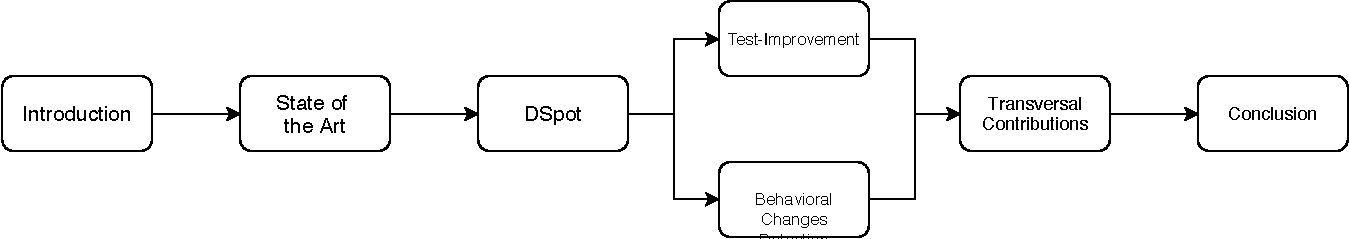
\includegraphics[width=\linewidth]{roadmap.pdf}}
	\caption{Dissertation Roadmap}
	\label{fig:intro:roadmap}
\end{figure}

This thesis is divided into 6 chapters.

First, \autoref{chap:sota} exposes the state of the art of test amplification.

Then, \autoref{chap:dspot} gives the detail of the major technical contributions of this thesis: \dspot.

\autoref{chap:test-improvement} and \autoref{chap:dci} relate two evaluations of \dspot on open-source projects from \gh.
Each of these evaluations has their own characteristics, novelties and motivations.

During my thesis, I developed a lot of skills that allowed me to participate to transversal contributions. 
These contributions are related in \autoref{chap:transversal-contributions}.

Eventually, I conclude and give the short- and long-term perspectives in \autoref{chap:conclusion}.

\autoref{fig:intro:roadmap} summarizes the roadmap.

\section{Software and Impact On The Community}
\label{sec:intro:software}

During my thesis, I developed strong artifacts to evaluate the approaches.
These artifacts are strong enough to be applicable on real code base such open-source projects from \gh or the STAMP partners' codebases.
This show strong evidence on the applicability and generalization of the results.
Following, the list of these artifacts and a small description.

\begin{itemize}
	\item[\dspot]\footnote{\url{https://github.com/STAMP-project/dspot.git}} is a test suite amplifier. 
	It takes as input a project and its test suite and will produce test cases according to a test criterion adequacy such as branch coverage or mutation score. 
	\item[DSpot-diff-test-selection]\footnote{\url{https://github.com/STAMP-project/dspot/tree/master/dspot-diff-test-selection}} is a maven plugin, based on OpenClover, that produces the list of test classes and their test methods that execute a provided diff.
	\item[DSpot-prettifier]\footnote{\url{https://github.com/STAMP-project/dspot/tree/master/dspot-prettifier}} aims a make better good looking amplified test methods obtained with \dspot. 
	It relies on several operations such as minimization, renaming local variables and test methods (based on code2vec)
	\item [Test-runner]\footnote{\url{https://github.com/STAMP-project/test-runner}} is a library that allows developer to execute test in a new and clean JVM. 
	\item[AssertFixer]\footnote{\url{https://github.com/STAMP-project/AssertFixer}} aims to fix the assertion in a test suite, using the program as specifications.
\end{itemize}

To maximize the artefacts' impact on the community, all of them are open-source and available on \gh.

\clearpage

\section{Publications}
\label{sec:intro:publications}

\renewcommand\bibname{~}
\vspace{-2.8cm}
\let\oldaddcontentsline\addcontentsline% Store \addcontentsline
\renewcommand{\addcontentsline}[3]{}% Make \addcontentsline a no-op
\begingroup
\let\clearpage\relax
\begin{thebibliography}{xxxx}
	\bibitem[Danglot~2019]{Danglot2019}
	Benjamin Danglot, Oscar~Luis Vera-P{\'e}rez, Benoit Baudry and Martin
	Monperrus.
	\newblock {\em Automatic test improvement with DSpot: a study with ten mature
		open-source projects}.
	\newblock Empirical Software Engineering, Apr 2019.
	
	\bibitem[Danglot~2019a]{DBLP:journals/corr/abs-1902-08482}
	Benjamin Danglot, Martin Monperrus, Walter Rudametkin and Benoit Baudry.
	\newblock {\em An Approach and Benchmark to Detect Behavioral Changes of
		Commits in Continuous Integration}.
	\newblock CoRR, vol.~abs/1902.08482, 2019.
	
	\bibitem[Vera-P{\'e}rez~2018]{descartes}
	Oscar~Luis Vera-P{\'e}rez, Benjamin Danglot, Martin Monperrus and Benoit
	Baudry.
	\newblock {\em A comprehensive study of pseudo-tested methods}.
	\newblock Empirical Software Engineering, Sep 2018.
	
	\bibitem[Danglot~2018]{Danglot2018}
	Benjamin Danglot, Philippe Preux, Benoit Baudry and Martin Monperrus.
	\newblock {\em Correctness attraction: a study of stability of software
		behavior under runtime perturbation}.
	\newblock Empirical Software Engineering, vol.~23, no.~4, pages 2086--2119, Aug
	2018.
	
	\bibitem[Danglot~2017]{survey:amplification}
	Benjamin Danglot, Oscar Vera{-}Perez, Zhongxing Yu, Martin Monperrus and Benoit
	Baudry.
	\newblock {\em The Emerging Field of Test Amplification: {A} Survey}.
	\newblock CoRR, vol.~abs/1705.10692, 2017.
	
	\bibitem[Yu~2019]{Yu2019}
	Zhongxing Yu, Matias Martinez, Benjamin Danglot, Thomas Durieux and Martin
	Monperrus.
	\newblock {\em Alleviating patch overfitting with automatic test generation: a
		study of feasibility and effectiveness for the Nopol repair system}.
	\newblock Empirical Software Engineering, vol.~24, no.~1, pages 33--67, Feb
	2019.
\end{thebibliography}
\endgroup
\let\addcontentsline\oldaddcontentsline% Restore \addcontentsline

